%Geometrické a objemové modelování. Hraniční metoda, metoda CSG, výčet prostoru, oktantové stromy.

\subsection{Geometrické a objemové modelování}
\begin{itemize}
	\item Geometrické modelování \textbf{zkoumá reálné objekty z hlediska geometrických vlastností}.
	\item Je to \textbf{soubor metod k popisu těles}. Rozlišujeme \textbf{3 základní typy modelů} (příklady jsou uvedeny pro \textit{trojboký hranol}):
	\begin{enumerate}
		\item \textbf{Drátěný model} --  je určen seznamem devíti \textbf{hran}.
		\item \textbf{Hraniční model} -- je určen seznamem pěti \textbf{stěn}.
		\item \textbf{Objemový model} -- je určen \textbf{velikostí stran podstavy} a \textbf{výškou} (CSG).
	\end{enumerate}
\item \textbf{Objemové reprezentace} těles nesou přímé informace o vnitřních objemech těles a používají se i jako pomocné datové struktury vzhledem k rychlému zpracování. Oproti tomu povrchové reprezentace těles nesou přímé informace o povrchu tělesa (např. hrany, stěny) a poměrně snadno se zobrazují.
\end{itemize}

\begin{figure}[H]
	\centering
	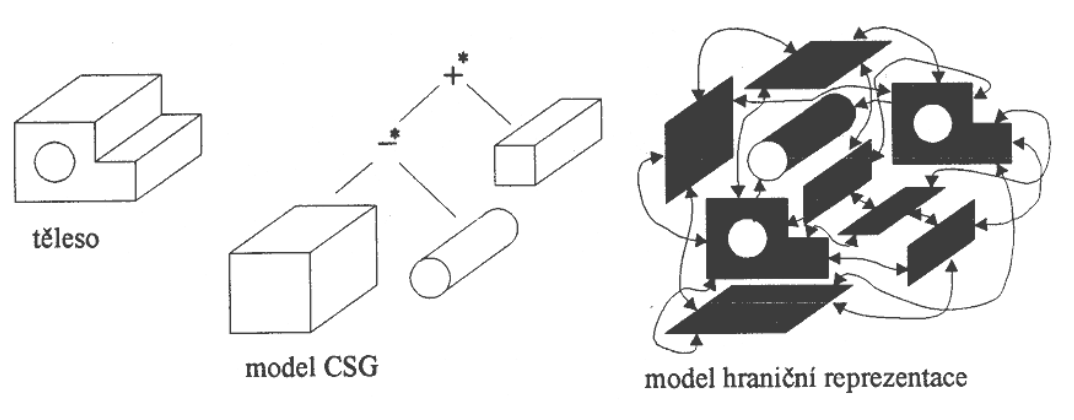
\includegraphics[width=0.8\textwidth]{assets/4_modely}
\end{figure}

\subsection{N-maniflod}
N-manifold v topologii představuje topologický prostor, který lokálně připomíná reálný n-dimenzionální prostor. N-manifold je takový topologický manifold, jehož \textbf{každý bod} má okolí homeomorfní s $\mathbb{R}^n$. V podstatě definuje hranice (\textbf{povrch}) tělesa.
\begin{itemize}
\item \textbf{1-manifold} je například kruh (nemá žádný povrch).
\item \textbf{2-manifold} (v 3D prostoru) je \textbf{povrch tělesa}, s kterým lze jednoduše manipulovat (rozdělit rovinou, naříznout (nová hrana)).
\item \textbf{3-manifold} (v 3D prostoru) je \textbf{povrch s dírami}, s tímto tělesem už se tak jednoduše nedá manipulovat.
\end{itemize}

\subsection{Drátěné (hranové) modely (wireframe model)}
\begin{itemize}
	\item Drátěné modely jsou reprezentovány \textbf{hranami objektu} a skládají se z \textbf{bodů}, \textbf{přímek} a \textbf{křivek}.
	\item První wireframe systémy byly pouze dvou-dimenzionální, používaly se především na návrhy tištěných spojů. Základními elementy těchto systémů byly body, přímky a oblouky některých kuželoseček. Vnitřní reprezentaci tvořil obvykle seznam úseček a oblouků.
	\item V 70. letech byla wireframe reprezentace použita i pro \textbf{modelování v prostoru}. Zde však vznikaly dost závažné \textbf{problémy}:
	\begin{itemize}
		\item možnost vytvoření nejednoznačných modelů,
		\item možnost vytvoření nesmyslných modelů,
		\item problém velkého počtu dat pro ,,drátěný'' popis objektu.
	\end{itemize}
	\item Průmět drátěného modelu může mít více významů.
	\item Pokud u modelu \textbf{vynecháme} některé \textbf{hrany}, dostaneme \textbf{nesmyslný} (nonsense) model.
	\item U wireframe modelů je velice obtížné kontrolovat jejich \textbf{logickou správnost}.
	\item Poslední nevýhodou je \textbf{značné množství dat}, které jsou nutné pro úplný popis objektu. 
	\item \textbf{Například:} obecně pro jednoznačné určení kvádru v prostoru stačí výška, šířka, hloubka a poloha. Wireframe model kvádru musí obsahovat souřadnice osmi vrcholů, musí být určeno dvanáct hran a ještě není model jednoznačný.
\end{itemize}

\begin{figure}[H]
	\centering
	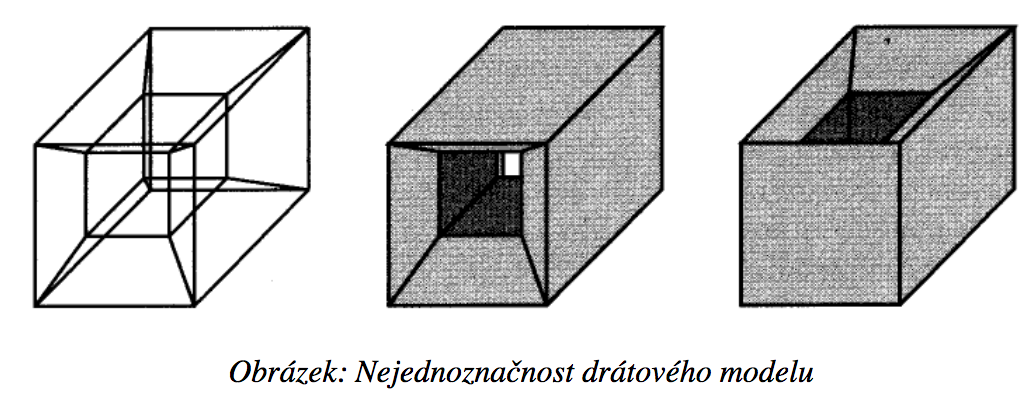
\includegraphics[width=0.6\textwidth]{assets/4_dratovy_model}
\end{figure} 

 \subsection{Hraniční metoda (hraniční model)}
 \begin{itemize}
 	\item Tato reprezentace patří k \textbf{nejpoužívanějším} typům při geometrickém popisu objektů.
 	\item Historicky vyžadovala hranici \textbf{2-manifold v E$3$}, což znemožňovalo použití např. těles, která se sama sebe dotýkají (obrázek dole vlevo). Na druhou stranu byly pro uvedenou třídu těles velice dobře prozkoumány topologické vlastnosti. Tento požadavek byl však později \textbf{revidován} (boleaovské operace nemohou zaručit výsledek v 2-manifold E$^3$, obrázek dole vpravo).
 	\item Metoda reprezentace tělesa pomocí hranice, spočívá v tom, že \textbf{těleso je dáno svou hranicí} (povrchem), která je \textbf{orientována} a dělí tedy prostor na dvě části - \textbf{vnitřek} tělesa a \textbf{vnějšek} tělesa.
 	\item Popis tělesa je rozdělen na dvě části:
 	\begin{itemize}
		\item \textbf{topologická} - popisuje vzájemné \textbf{vztahy} mezi entitami tělesa (vztahy mezi stěnami, hranami a vrcholy),
		\item \textbf{geometrická} - popisuje \textbf{umístění} entit tělesa v \textbf{prostoru} (souřadnice prostorů, rovnice ploch, ...).
 	\end{itemize}
 	\item Těleso je definováno těmito informacemi:
 	\begin{itemize}
		\item	\textbf{seznam povrchů (shell)}, které těleso omezují,
		\item	\textbf{seznam stěn (face)} definující povrch tělesa,
		\item	\textbf{seznam smyček (loop)}, které definují stěny. Jde o \textbf{orientované hrany}. Obsahuje-li stěna jednu smyčku, jde o stěnu bez děr. Je li dána více smyčkami jsou ve stěně tunely. \textbf{Směr rotace} smyčky udává \textbf{normálu} stěny a určuje tedy na které straně stěny je \textbf{vnitřek} tělesa a která strana je \textbf{vnější} (smyčka proti směru hodinových ručiček – stěna z vnějšku). Je‑li uprostřed stěny, jde o díru (tunel).
		\item	\textbf{seznam hran (edge)} definující smyčky.
 	\end{itemize}
 	\item Né všechny uvedené informace (o dírách, stěnách atd) musí být explicitně zaznamenány v datové struktuře, je však žádoucí aby je bylo možné \textbf{rychle dopočítat}.
 	\item Jednou z hraniční reprezentací těles je datová struktura zvaná \textbf{okřídlená hrana} daná hranou a dvěma plochami k ní přiléhajícími.
 \end{itemize}

\begin{figure}[H]
	\centering
	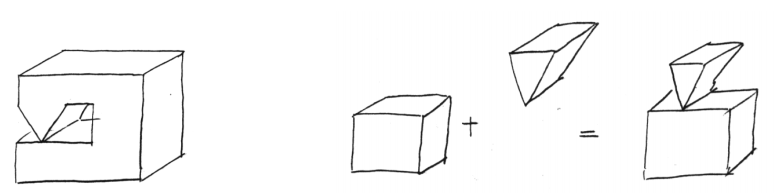
\includegraphics[width=0.6\textwidth]{assets/4_hranicnic_manifold}
\end{figure} 

\subsubsection{Okřídlená hrana}
Okřídlená hrana je \textbf{datová struktura} pro reprezentaci polygonových modelů taková, že jasně definuje jejich geometrii a topologii stěn, hran a vrcholů.

\begin{itemize}
\item Umožňuje jednoduchý průchod po jednotlivě spojených hranách, stěnách a bodech díky vzájemně propojeným strukturám.
\item Okřídlené hraně přiléhají 2 stěny \textbf{nalevo} a \textbf{napravo} od ní. Zároveň si uchovává informaci o \textbf{následujících} a \textbf{předcházejících} hranách podél každé ze stěn, které jsou uspořádány po směru hodinových ručiček.
\end{itemize}

\begin{figure}[H]
\centering
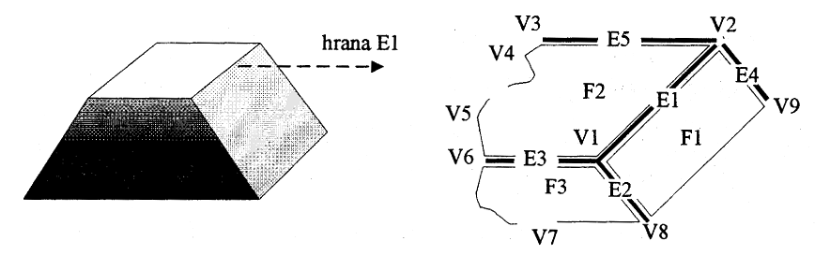
\includegraphics[width=0.5\textwidth]{assets/4_okridlena_hrana}
\end{figure} 

\subsubsection{Eulerovy operátory hraniční reprezentace}
Slouží k obsluze datových struktur hraniční reprezentace. Modifikují datovou strukturu tak, aby vždy popisovala nějaké těleso (jinými slovy, lze pomocí nich vytvářet nová tělesa). Pro jednoduché mnohostěny (uzavřené bez otvorů) platí následující \textbf{Eulerova formule}:
\begin{equation*}
V + F - E = 2,
\end{equation*}

kde $ V $ je počet vrcholů, $ E $ je počet hran a $ F $ je počet stěn. Pro mnohostěny s otvory platí \textbf{zobecněná Eulerova formule}:
\begin{equation*}
V + F - E = H + 2(B - P),
\end{equation*}

kde $ B $ (Body) je počet disjunktních částí tělesa, $ H $ (Hole) je počet otvorů ve stěnách a $ P $ (Passage) je počet děr v tělese.

\begin{itemize}
	\item \textbf{Základní operace} -- \texttt{createSolid} (vytvoří minimální neprázdné těleso), \texttt{splitEdge} (rozdělí zadanou hranu vložením nového vrcholu), \texttt{splitFace} (rozdělí zadanou stěnu vložením nové hrany).
	\item \textbf{Další operace} -- \texttt{splitSolid} (provede řez nějakého tělesa ořezovou rovinou).
\end{itemize}

\begin{figure}[H]
	\centering
	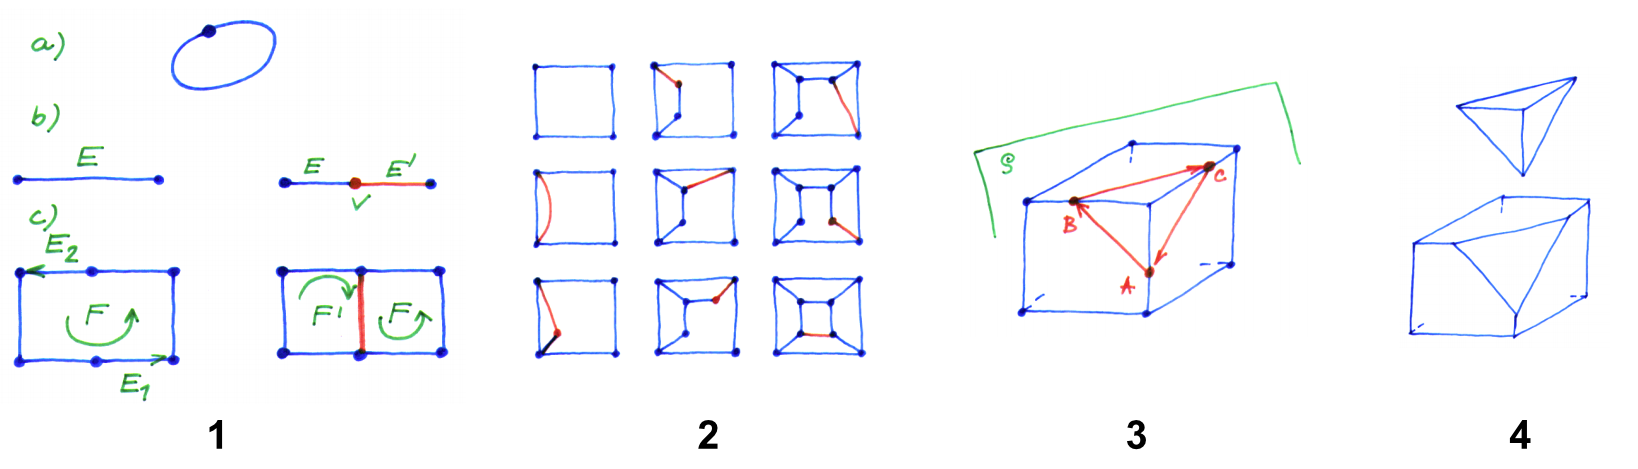
\includegraphics[width=0.9\textwidth]{assets/4_hranicni_euler}
\end{figure} 

\textbf{Příklad:} Na obrázku výše (číslo 2) je postup vytvoření kvádru. Nejprve se zavolá \texttt{createSolid} a pak $3 \times$ \texttt{splitEdge} $\rightarrow$ tím výchozí výsledek čtverec (vlevo nahoře). Dále se pak střídá použití operátorů \texttt{splitFace} a \texttt{splitEdge} dokud není vytvořena taková struktura hran a vrcholů jako obrázek vpravo dole.

 \subsection{Metoda CSG (objemový model)}
 \begin{itemize}
 	\item \textbf{Constructive Solid Geometry} je metoda reprezentace těles, kdy jsou tělesa tvořena za pomocí standardních \textbf{primitivních těles} (kvádr, hranol, válec, kužel, koule, toroid, …), \textbf{regularizovaných booleovských operací} a \textbf{geometrických transformací}.
	\item Uživatel si naskládá primitivní (či dříve vytvořené) tělesa do prostoru a aplikuje na ně boolovské operace jako sjednocení, průnik, rozdíl, čímž vznikne nový útvar.
	\item Z hlediska \textbf{datové struktury} jsou tělesa popsány stromem. \textbf{Listy} stromu odpovídají primitivním tělesům a transformacím, vyčteme z nich tedy rozmístění a velikosti těles. Zbylé uzly tvoří \textbf{boolovské operace} které jsou nad tělesy vykonány.
	\item CSG strom je \textbf{binární}, pokud chápeme boolovské operace jako binární, jinak tomu být nemusí.
		\begin{figure}[H]
		\centering
		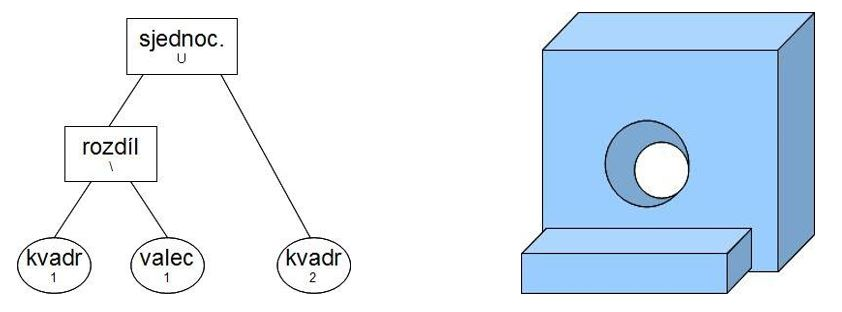
\includegraphics[width=0.6\textwidth]{assets/4_csg}
		\end{figure}
 	\item Výhoda stromové struktury je že uchovává \textbf{historii} modelace tělesa, kterou lze využít při další úpravě.
 	\item Další výhodou CSG tohoto přístupu je \textbf{jednoduchost boolovských operací}.
 	\item Na rozdíl od hraniční metody, není třeba náročného výpočtu hranic nového tělesa.
 \end{itemize}

 \subsection{Výčet prostoru - BSP stromy}
 Při vykreslování objektů v prostoru narazíme na problém co vykreslit dřív a co později, aby to co je blíže pozorovateli překrývalo to co je od něj dál. Nejjednodušším algoritmem je \textbf{malířův algoritmus}, ten postupně vykresluje objekty seřazené od nejvzdálenějšího k nejbližšímu. Na obrázku (1) níže je však ukázaný problém, s kterým si neporadí. Toto řeší BSP stromy.
 
\textbf{BSP strom} je binární strom nesoucí informaci o rozdělení prostorů. Představuje \textbf{hierarchické rekurzivní} dělení N-dimenzionální prostoru na konvexní podprostory. BSP stromy uchovávají toto rozdělení tak že vlevo je \textbf{horní poloprostor} a vpravo \textbf{dolní poloprostor} (obr dole č. 3). Každý poloprostor poté obsahuje množinu objektů, které se v něm nachází.

\begin{figure}[H]
	\centering
	\includegraphics[width=0.8\textwidth]{assets/4_Bsp}
\end{figure}
 
 \subsection{Oktantové stromy}
 \begin{itemize}
 	\item Jedna z metod objemového modelování.
 	\item Těleso je definováno \textbf{objemovými elementy} (\textbf{voxel}), což je v podstatě 3D pixel. Jde o \textbf{malé krychličky}, na které je rozdělen prostor a které buď jsou v tělese nebo nejsou.
 	\item Na obrázku níže je zobrazen tento způsob pro 2D. Zápis takového 2D tělesa by mohl vypadat takto: [0, 0, false], [0, 1, true], [0, 2, true], ...
	\item Čím \textbf{jemnější detaily} potřebujeme modelovat, tím jemněji potřebujeme plochu rozdělit.
	\item Jenže tím se nám taky \textbf{zvedají nároky na paměť}. Proto zavádíme \textbf{oktanové stromy}, které tento problém eliminují.
		\begin{figure}[H]
		\centering
		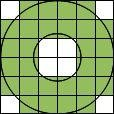
\includegraphics[width=0.2\textwidth]{assets/4_octan}
		\end{figure}
\end{itemize}

\subsubsection{Struktura oktantových stromů}
\begin{itemize}
	\item Oktantové stromy \textbf{zmenšují paměťovou náročnost} detailních modelů, tak že zjemní pouze elementy, kterých se detail týká.
	\item Začíná se tedy na velkých voxelech, ale ty nyní mohou nabývat třech stavů:	
	 \begin{itemize}
			\item voxel je obsažen v tělese
			\item voxel není obsažen v tělese
			\item voxel je částečně obsažen v tělese.
	\end{itemize}
	\item V dalším kroku se řeší ty voxely, které jsou nerozhodné, tedy částečně obsaženy v tělese. Takový voxel ležící na hranici tělesa \textbf{rozdělíme na osm menších voxelů}. (Na obrázku níže je tento postup znázorněn ve 2D prostoru, kde rozdělíme na 4 pixely).
		\begin{figure}[H]
		\centering
		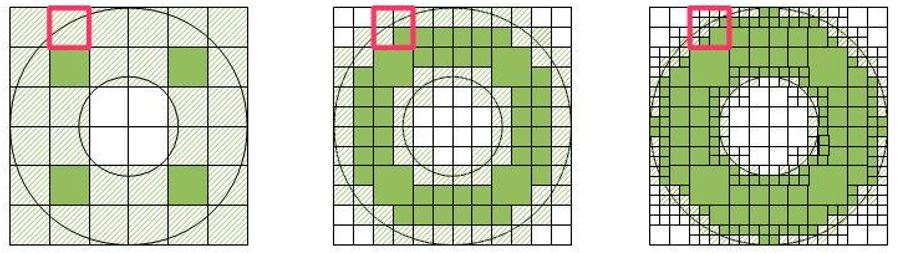
\includegraphics[width=0.6\textwidth]{assets/4_octan2}
		\end{figure}
	\item Výsledná struktura je pak zapsána do \textbf{oktanových stromů} (stromy s max. osmi větvemi). Dole máme oktanový (respektive kvartálový, protože jsme jen v 2D prostoru) strom popisující oblast, která je vyznačená červeně na obrázku výše.
		\begin{figure}[H]
		\centering
		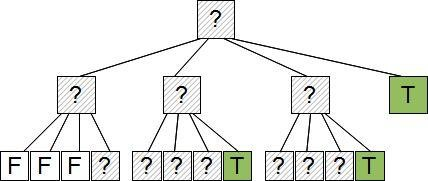
\includegraphics[width=0.5\textwidth]{assets/4_octan_struct}
		\end{figure}
\end{itemize}
